\chapter{Wybór stosowanych technologii}
\section{Język C++11 oraz wybór kompilatora}
Aplikacja została napisana z użyciem języka C++11. Język ten
wybrano z kilku powodów. Skorzystano tu z jego natury jako języka zorientowanego obiektowo. Dzięki temu podczas wykonania programu stworzono klasy odpowiadające obiektom w świecie realnym - elektrony, pułapki elektronowe itp.
Kolejnym powodem dla którego wykorzystano język C++ jest jego wydajność. Kod napisany
w języku C++ jest kompilowany bezpośrednio i w pełni do kodu maszynowego  wykonywanego przez procesor komputera. Dzięki temu
otrzymujemy maksymalną możliwą wydajność inaczej niż gdy używamy innych
obiektowych języków programowania wysokiego poziomu, które są kompilowane do kodu
zarządzanego (tzw. kodu bajtowego na przykład w przypadku Javy) gdzie dodatkowy narzut
generowany jest przez warstwę pośrednią w postaci maszyny wirtualnej. 

C++11 jest standardem języka C++ zastępującym standard C++03. Wprowadza on kilka dodatków do rdzenia języka oraz znacznie rozszerza bibliotekę standardową C++. Dla przykładu wprowadza on słowo kluczowe \textit{auto} jako zastępczy typ zmiennej, który zostanie wydedukowany na podstawie wartości za pomocą której zmienna zostanie zainicjalizowana. Nowa biblioteka wprowadza również kilka silników do generacji liczb pseudolosowych. W projekcie wykorzystano generator oparty na jednostajnie ciągłym rozkładzie prawdopodobieństwa.

Do kompilacji użyto darmowego kompilatora GCC (Gnu Compiler Collecion), konkretnie jego implementacji dla platformy Windows - MinGW w wersji 3.2.2 (Minimalist GNU for Windows).

\section{Środowisko programistyczne}

Program był tworzony z użyciem wieloplatformowego zintegrowanego środowiska programistycznego języków C/C++ - \textbf{CLion} (wersja 2016.2.3) produkcji spółki JetBrains. Było to podyktowane głównie znajomością produktów firmy JetBrains. \href{https://www.jetbrains.com/clion/}{CLion} jest produktem komercyjnym, jednak skorzystano tu z darmowej licencji studenckiej. IDE produkcji JetBrains obsługuje również 	system zarządzania kompilacją \textbf{CMake}, którego główną cechą jest niezależność od używanego kompilatora oraz platformy sprzętowej - CMake nie kompiluje programu samodzielnie, lecz tworzy pliki z regułami kompilacji dla konkretnego środowiska.

\begin{figure}[h]
\centering
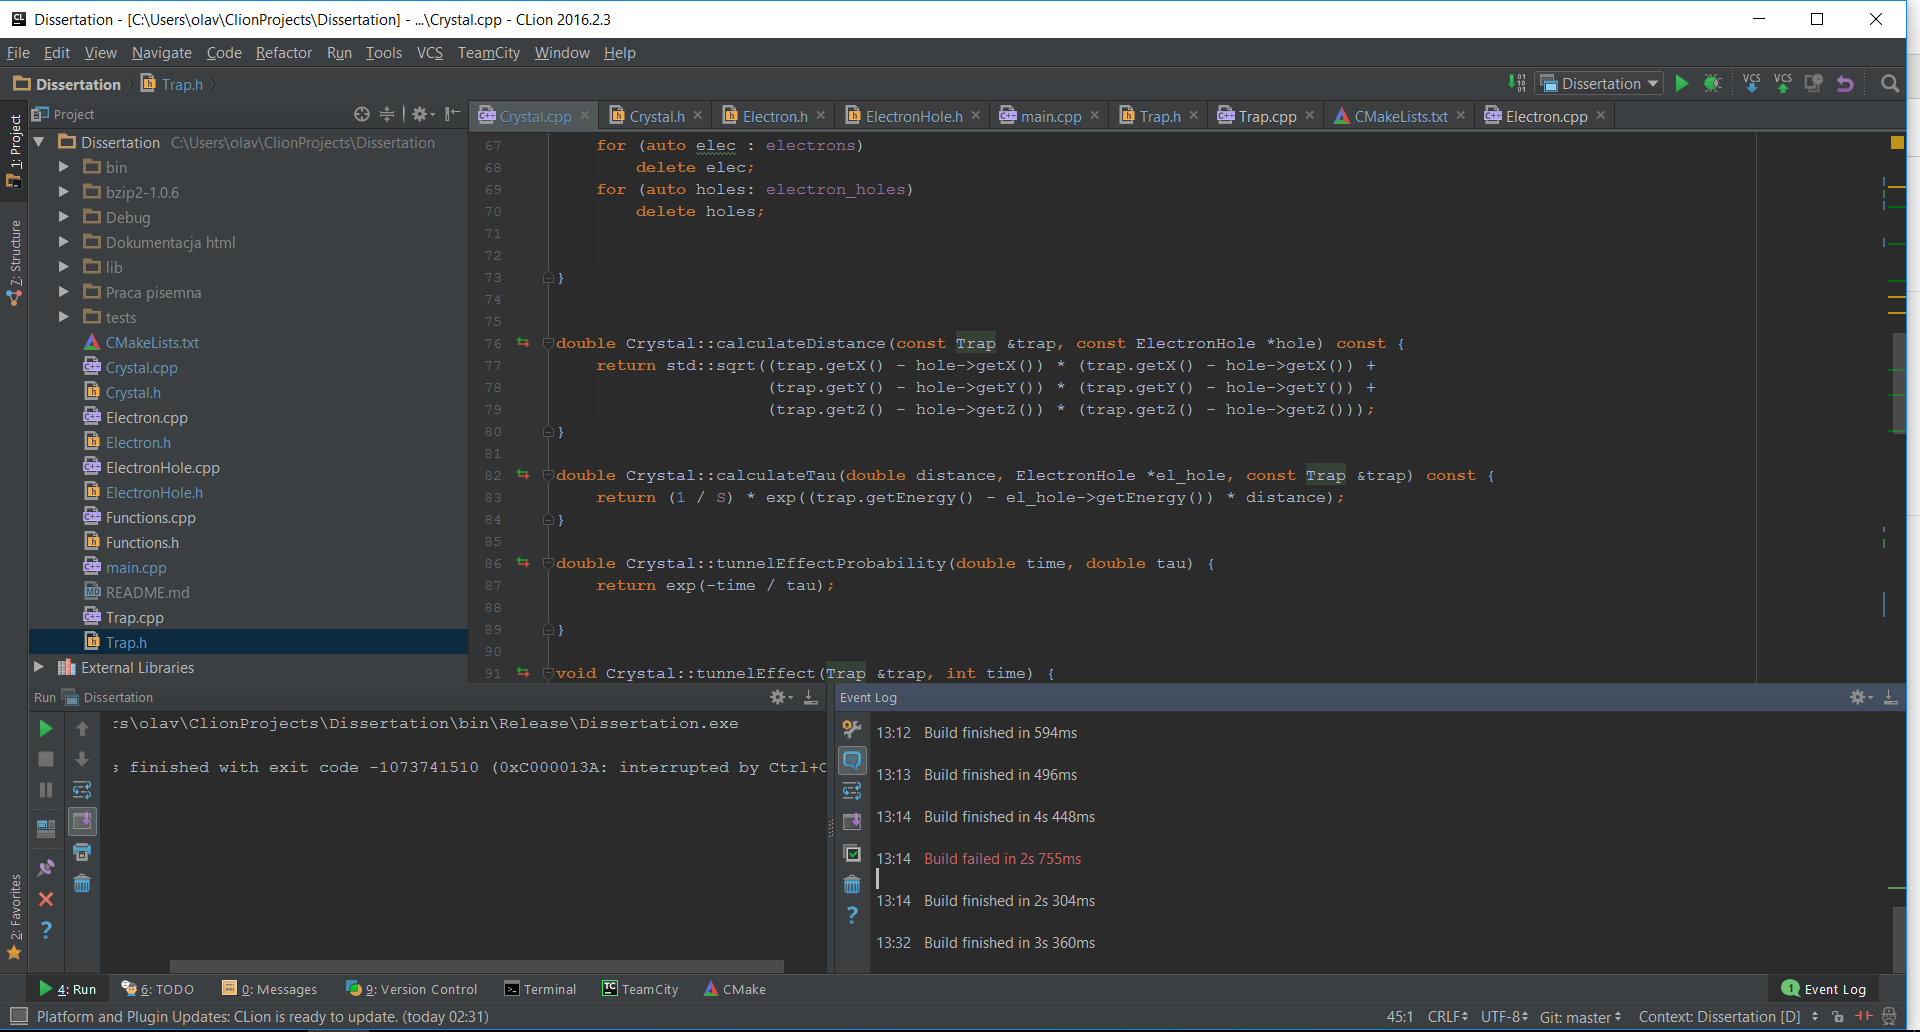
\includegraphics[width=17cm]{clion}
\caption{Wygląd okna programu CLion \cite{struktura_pasmowa}}
\label{fig:clion}
\end{figure}

Dużą zaletą podczas pracy z IDE produkcji JetBrains jest jego intuicyjna i prosta obsługa całości projektu. Dodatkowo, CLion posiada możliwość bezpośredniego połączenia projektu z wybranym serwerem kontroli wersji co uprościło pracę nad projektem. Z racji tego, że w chwili obecnej program do kompilacji używa tylko systemu CMake, niezbędne było nauczenie się jego obsługi  oraz odpowiedniej składni.

\section{System kontroli wersji Git}

System kontroli wersji śledzi wszystkie zmiany dokonywane w plikach i umożliwia przywołanie dowolnej wcześniejszej wersji. Jest to przydatne narzędzie w łączeniu zmian dokonanych przez wiele osób w różnym czasie.

W procesie tworzenia aplikacji wykorzystano system kontroli wersji Git oraz darmowy hostingowy serwis internetowy \href{https://github.com/}{GitHub}.
Głównym powodem wykorzystania tego systemu była jego popularność oraz prostota użytkowania.
System kontroli wersji okazał się być niezwykle użytecznym narzędziem pozwalającym na
śledzenie zmian w kodzie, wprowadzanie testowych rozwiązań bez
ryzyka zniszczenia kodu. Cały projekt można pobrać ze strony:
\begin{center}
\url{https://github.com/Sharkuu/Dissertation}
\end{center}

\section{Wizualizacja wyników - Gnuplot}

Po wygenerowaniu danych, aby z wizualizować wykres obrazujący zmianę ilości elektronów znajdujących się w stanie wzbudzonym (znajdujących się w pułapkach) wraz z upływem czasu skorzystano z programu \href{http://www.gnuplot.info/}{\textbf{Gnuplot}}.

Gnuplot jest narzędziem do kreślenia wykresów 2D i 3D, sterowanym z wiersza poleceń. Ta jego cecha, oraz możliwość pobierania zewnętrznych danych, umożliwia jego wykorzystanie do wizualizacji wyników z innych programów. Możliwe są dwa tryby pracy:
\begin{itemize}
\item Jezeli uruchomimy program bez podania zadnych parametrow (polecenie gnuplot), bedzie on pracowal w trybie interaktywnym (bedzie oczekiwal na komendy uzytkownika i kolejno je wykonywal). Aby zakonczyc prace, nalezy wpisac komende exit, quit lub q.
\item Jezeli podamy parametr (polecenie gnuplot plik), program wykona polecenia zawarte w pliku i zakonczy prace (tryb wsadowy)
\end{itemize}
